\clearpage
\setcounter{page}{1}
% \maketitlesupplementary


\section{Supplementary}
\label{sec:Supplementary}

\subsection{More Qualitative Comparison}
\label{More Qualitative Comparison}
VMix decouples aesthetic knowledge from content knowledge and introduces a novel conditional control method. To further verify its effectiveness, we provide additional experimental results here.

\noindent \textbf{Training Stability.} In \cref{sec:Methodology}, we introduced Value-Mixed Cross-Attention(vmix cross-attention), which learns a single value for the projected aesthetic embedding. This approach might seem counterintuitive, particularly since in the aesthetic branch, the Q (Query) and V (Value) originate from different sources. In practice, AesEmb is initialized from the [CLS] tokens of the text model, ensuring semantic alignment with the original text embedding. Furthermore, the projected aesthetic embedding must pass through a zero-initialized linear layer before it can finally enter the vmix cross-attention. This process further ensures a gentle injection of aesthetic knowledge, minimizing disruption to the original model. As shown in \cref{Figure 100}, the entire training process is relatively stable, with gradual improvements in lighting, color, and other visual aspects.

\noindent \textbf{Effect of VMix Cross-Attention.} In vmix cross-attention, we designed the aesthetic branch and the content branch to share the same attention map, denoted as $\mathbf{Q} \mathbf{K_c}^T$, to prevent the injection of aesthetic knowledge from significantly impairing the model's text fidelity capabilities. As demonstrated in \cref{Figure 101}, VMix produces an attention score map that closely resembles that of the baseline. After the denoising process, we can obtain a generated image that maintains a layout roughly equivalent to the baseline but with enhanced quality. This indicates that our vmix cross-attention allows the model to concentrate more on refining overall details, thereby directly boosting the model's performance across various fine-grained aesthetic dimensions, including lighting, color, and more.

\noindent \textbf{Comparison with LoRA.} Although in \cref{sec:Experiments}, we compared our method with SFT and textual inversion on the same dataset, the use of LoRA in our training process might obscure the enhancement of the final results. To clarify this, we trained a model with only LoRA on the same dataset. As shown in \cref{Figure 102}, our method significantly improves upon the SD~\cite{rombach2022high} more than the approach that uses only LoRA for training.

\begin{figure}[ht]
\centering
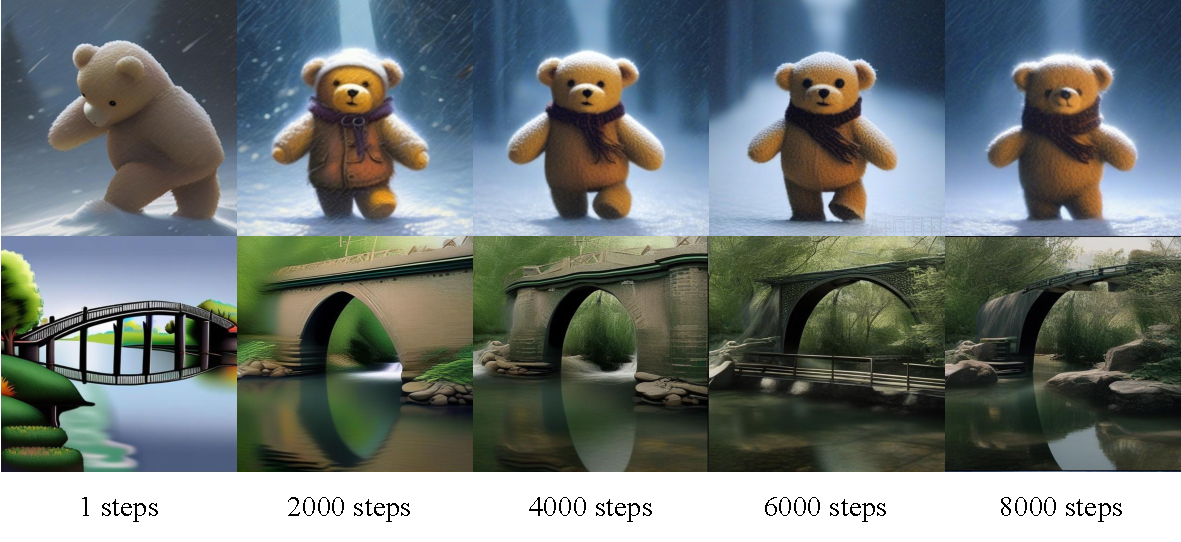
\includegraphics[scale=0.4]{sup_fig1.pdf}
    \caption{Visualization results of different training steps. Prompts: (1) A teddy bear walking in the snowstorm. (2) A bridge is depicted in the water.}
    \label{Figure 100}
\end{figure}

\begin{figure}[ht]
\centering
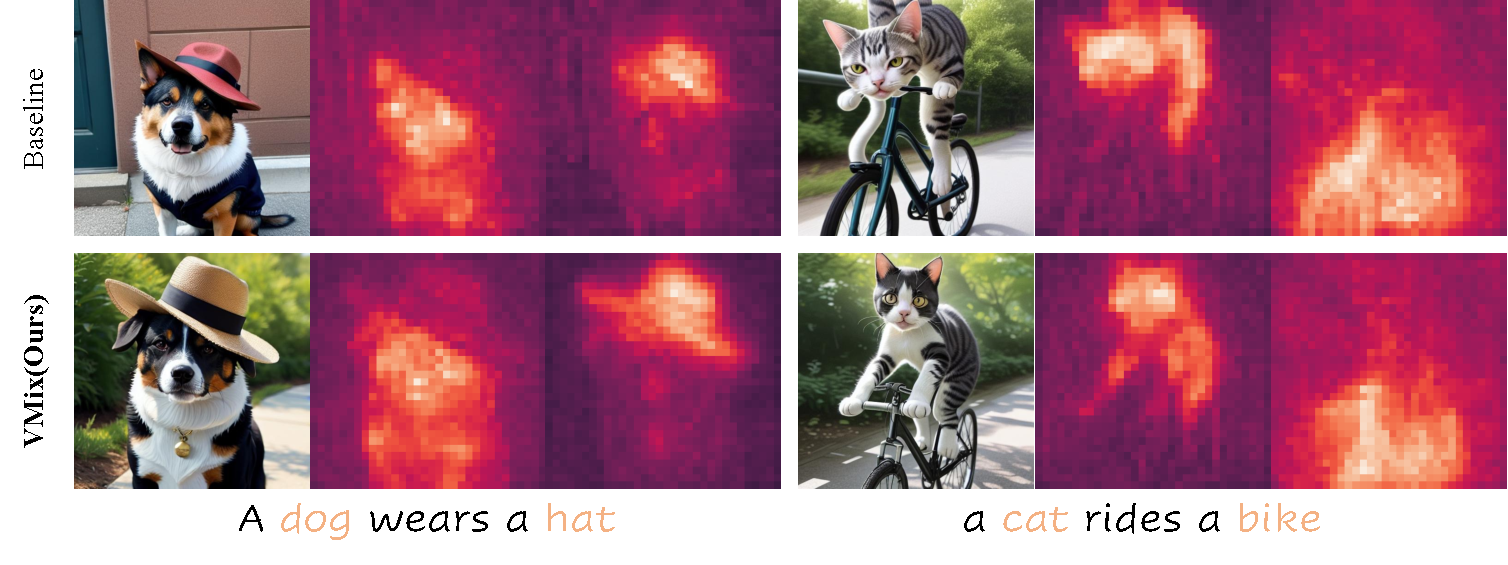
\includegraphics[scale=0.33]{sup_fig2.pdf}
    \caption{Visualization results of attention maps. VMix is capable of maintaining attention maps that closely resembles that of the baseline(SD~\cite{rombach2022high}) while further enhancing the quality of the generated images.}
    \label{Figure 101}
\end{figure}

\begin{figure}[ht]
\centering
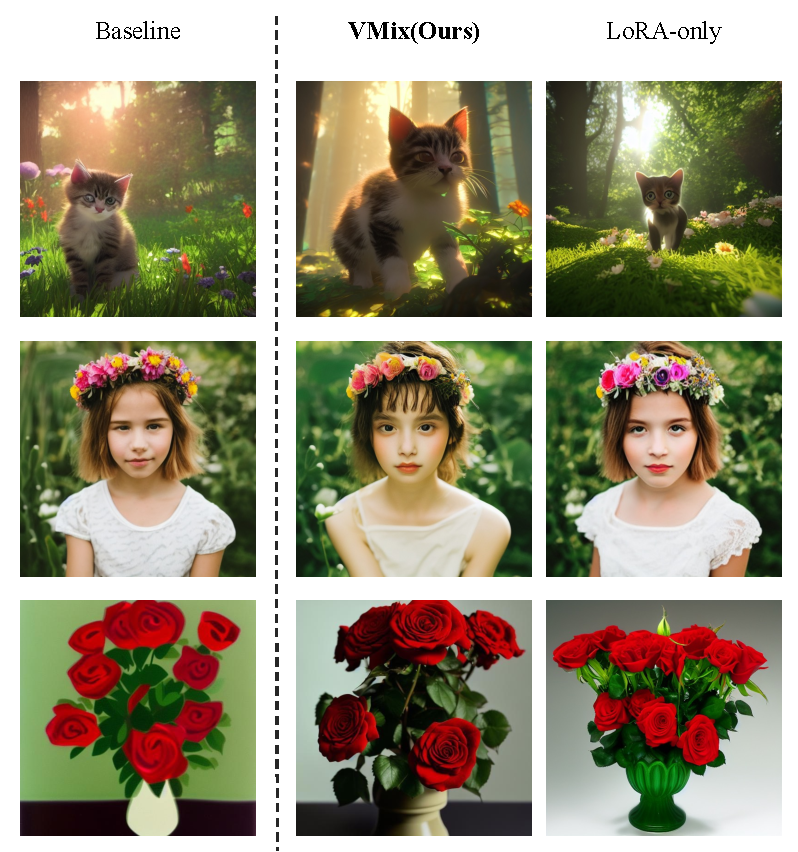
\includegraphics[scale=0.58]{sup_fig3.pdf}
    \caption{Qualitative comparison. Prompts: (1) Kitten in the forest with flowers with sunlight on them, Cinematic lighting, Unreal Engine 5. (2) Close-up of a young girl wearing a flower crown in the garden, portrait. (3) A green vase with several red roses in it.}
    \label{Figure 102}
\end{figure}

\subsection{More Visualization}
We apply VMix with ControlNet\cite{zhang2023adding} and IP-Adapter~\cite{ye2023ip}. As shown in \cref{Figure 104}, VMix can be compatible with these standard methods and generates images with better visual aesthetics. As shown in the \cref{Figure 105}, we have provided additional comparative results with SDXL~\cite{podell2023sdxl} as well as its variants. When VMix is incorporated, the generated results show significant improvements across various aesthetic dimensions, offering enhanced visual performance.

\begin{figure}[ht]
\centering
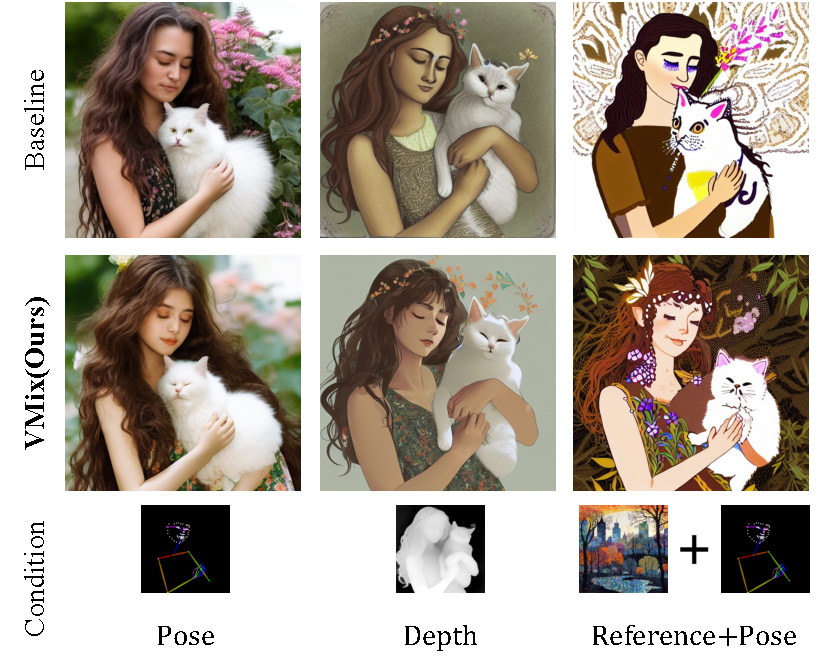
\includegraphics[scale=0.58]{sup_fig5.pdf}
    \caption{Qualitative results about VMix with ControlNet\cite{zhang2023adding} and IP-Adapter~\cite{ye2023ip}. Prompt: a young woman with long, wavy brown hair. she is wearing a sleeveless floral dress with a pattern of various flowers and leaves. the woman is holding a white, fluffy cat close to her face, seemingly in a moment of affection and joy. her eyes are closed, suggesting she is savoring the moment.}
    \label{Figure 104}
\end{figure}

\begin{figure*}[t]
\centering
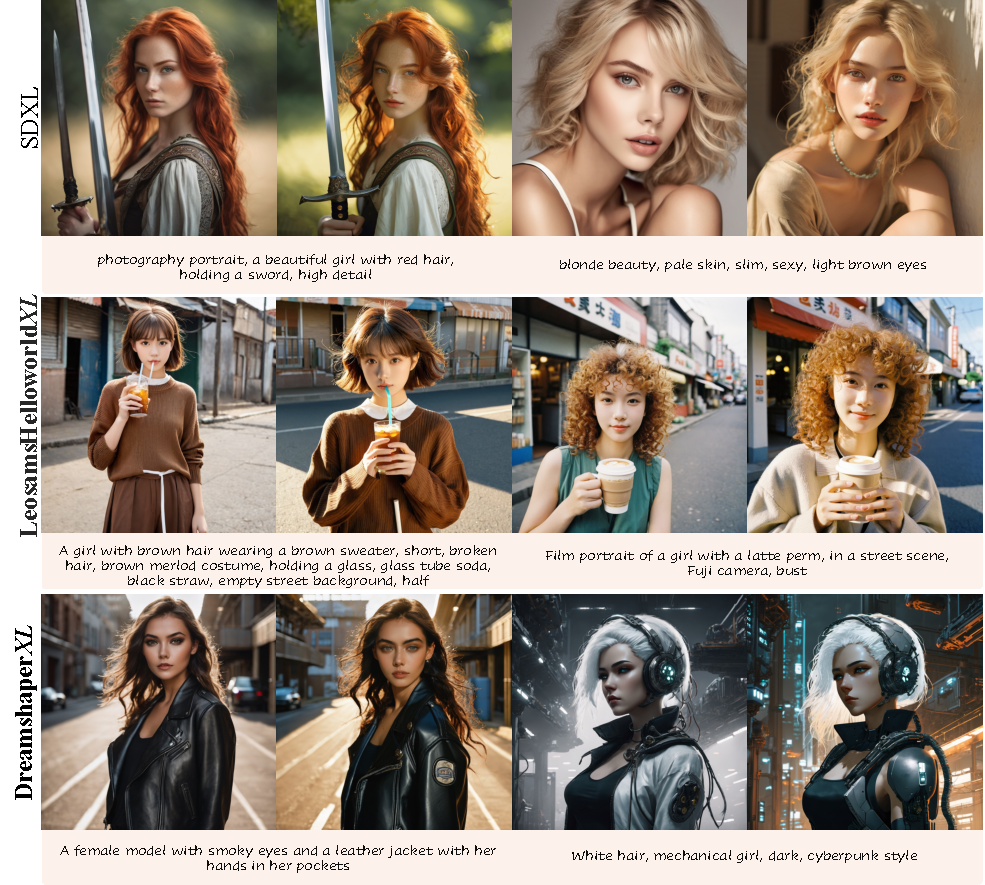
\includegraphics[scale=0.995]{sup6.pdf}
    \caption{Qualitative comparison between results with VMix(on the right) and without VMix(on the left), shows that VMix significantly enhances the quality of image generation.}
    \label{Figure 105}
\end{figure*}

\begin{figure*}[t]
\centering
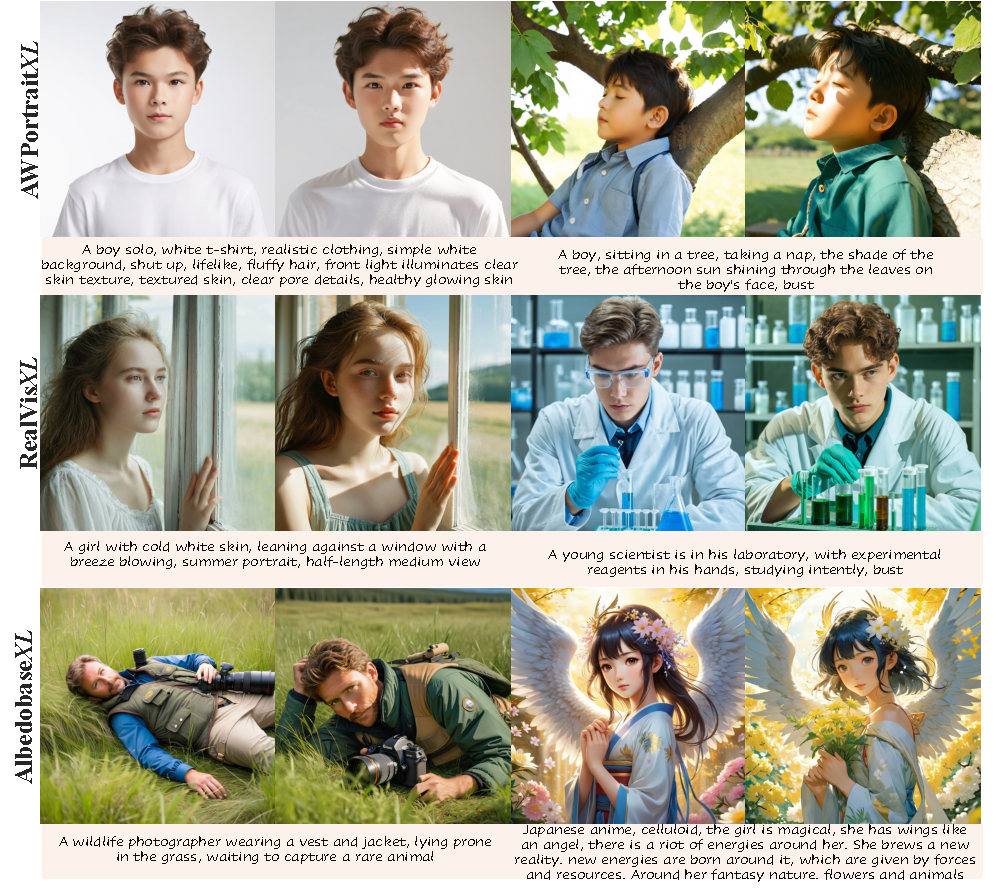
\includegraphics[scale=0.995]{sup7.pdf}
    \caption{Qualitative comparison between results with VMix(on the right) and without VMix(on the left), shows that VMix significantly enhances the quality of image generation.}
    \label{Figure 106}
\end{figure*}


\subsection{Limitations}
\label{Limitations}
Despite the superior aesthetic generation effects achieved by VMix, it still has several limitations: (1) Currently, the aesthetic labels form a closed set, and the included aesthetic dimensions may not cover all necessary aspects. Although we have confirmed the effectiveness of our current method, VMix's performance is inevitably impacted. We intend to further optimize this aspect in our future work. (2) Images generated by VMix may exhibit a bias towards certain specific objects. For instance, when we attempt to generate concrete objects found in real life, such as cups or mobile phones, and include all aesthetic labels, including emotional ones, during the inference phase, the resulting images might unexpectedly depict humans. This is because, in the training set, emotional labels are typically associated only with people or animals. Consequently, these labels may become bound to specific entities during the training phase, potentially affecting the outcomes of the inference process.
% Training stability
% VMix attention
% compare with LoRA 
% (inference time)

% with freeu/dpo
% with controlnet/ipa
% 更多关于aes emb的作用case
% results with more model

% limitations

% label是个闭集,会影响性能
